%TEX program = xelatex
\documentclass[letterpaper,10pt]{article}
\usepackage{amsmath}
\usepackage{hyperref}
\usepackage[margin=2cm]{geometry}
\usepackage{graphicx}

\begin{document}
\title{Performance of ESPO-R5 v1.0}
\author{Pascal Bourgault, Travis Logan, Trevor J. Smith, Juliette Lavoie}
\maketitle

The bias-adjustment performance assessment for ESPO-R5 was inspired by the "VALUE" project(\cite{Maraun2015}), a framework for evaluating different bias-adjustment and downscaling methods, like the Detrended Quantile Mapping (DQM) method used here (see \emph{adjustment.pdf}).
This framework defines a large collection of "properties" (VALUE calls them "indices") to study different aspects of the data, which can be compared to each other with "measures".
Through an implementation of a subset of these properties and measures into xclim, we looked at the changes brought about by the bias-adjustment for many different aspects of the data.
Following the "VALUE" project, we define four (4) different aspects: marginal, temporal, multivariate, and spatial. Table~\ref{tab:props} lists all properties studied for this analysis.
In addition to those reference-period diagnostics, we looked at the climate change signal and the ensemble variability.

\begin{table}[!ht]
    \centering
    \caption{Properties used in the performance assessment of ESPO-R5v1.0. All properties are compared with the simple "bias" measure, except the relative amplitude of the annual cycle (see footnote). All properties were computed on the full 30 years of daily data, except the means which were computed seperately for each month.}
    \begin{tabular}{l|c|c|c|l}
    \hline
    Property                               & Short name & Variables          & Aspect   & Source \\ \hline
    Mean                                   & mean       & tasmin, tasmax, pr & marginal & VALUE \\ \hline
    First percentile                       & q01        & tasmin, tasmax     & marginal & VALUE \\ \hline
    95th percentile                        & q95        & pr                 & marginal & VALUE \\ \hline
    99th percentile                        & q99        & tasmin, tasmax, pr & marginal & VALUE \\ \hline
    Dry spell frequency                    & dry\_spell\_freq & pr           & marginal & VALUE \\ \hline
    Amplitude of the annual cycle          & aca        & tasmin, tasmax     & temporal & VALUE \\ \hline
    Relative amplitude of the annual cycle & aca        & pr                 & temporal & VALUE \\ \hline
    Lag-1 autocorrelation                  & lag1       & tasmax             & temporal & VALUE \\ \hline
    Inter-variable correlation (spearman)  & corr       & tasmin-tasmax, pr-tasmax & multivariate & VALUE \\ \hline
    Spatial correlograms                   & correlogram & tasmin, tasmax, pr & spatial & \cite{Francois2020} \\\hline
    Principal empirical orthogonal function& first\_eof & tasmin, tasmax, pr & spatial & \cite{Vrac2018} \\ \hline
    \end{tabular}
    \label{tab:props}

\end{table}

The \emph{properties} were computed for the calibration period (years 1981-2010) for the raw simulations, the bias-adjusted scenarios, and the reference (ERA5-Land).
The results for the raw simulations were compared to those for the reference using a \emph{measure} appropriate for the respective property.\footnote{All properties in \ref{tab:props} were compared using a simple bias measure ($P_{sim} - P_{ref}$) except for the \emph{relative amplitude of the annual cycle}, which used the ratio measure ($P_{sim} / P_{ref}$)}. This way, for each member of the ensemble, one can visualize a given property and compare the measures to assess the improvement brought by the bias adjustment. Because of performance issues, the properties and measures were not computed on the full domain of ESPO-R, but rather on three smaller regions chosen to cover different climate types. These are shown in figure~\ref{fig:map}.

\begin{figure}
    \centering
    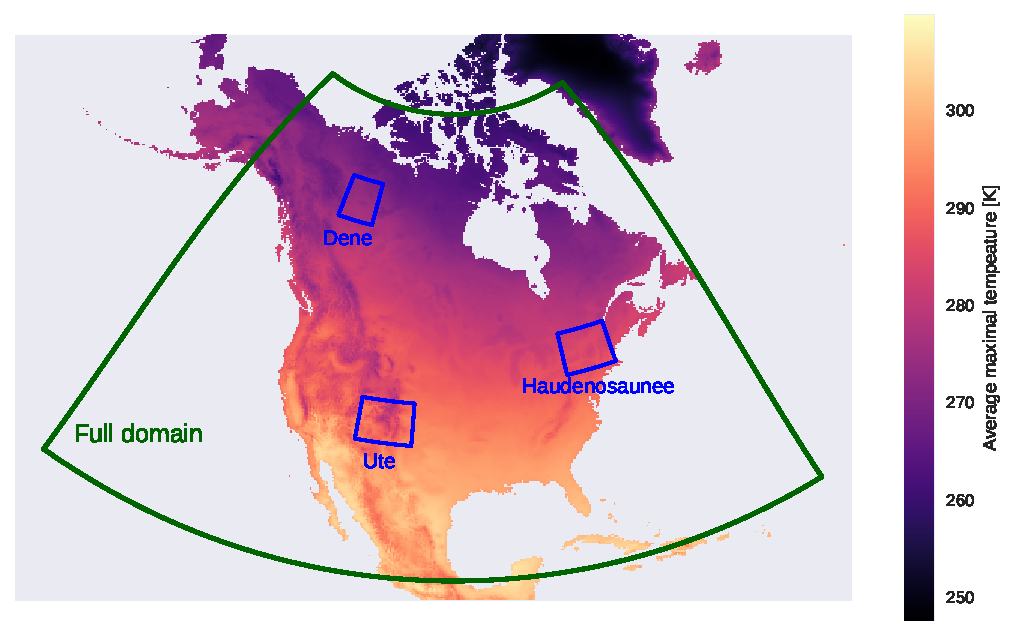
\includegraphics[width=0.75\textwidth]{../images/regions_domain_map.pdf}
    \caption{Map showing the domain of ESPO-R5v1.0 and the three diagnostics regions used in this study. All three regions have the same number of points, their size varies on this figure because of its rotated pole projection.}\label{fig:map}
\end{figure}

To complement this useful but quite exhaustive collection of maps, the proportion of improved grid points (we'll call this indicator IMP) was found for each property.
A grid point is said to have been improved if the bias (ratio) between the scenario and the reference is smaller (closer to 1) than the one between the raw simulation and the reference.
By taking the mean across all members of the ensemble, this allowed us to have an idea of which properties were improved by the bias adjustment (those with IMP close to 100 \%), which were not impacted (IMP around 50\%), and which were worsened (IMP smaller than 50 \%).
Fortunately, we found almost no properties of the latter case in this study. Figure~\ref{fig:imp} shows a heat map of those IMP values for each member and properties.

\begin{figure}
    \centering
    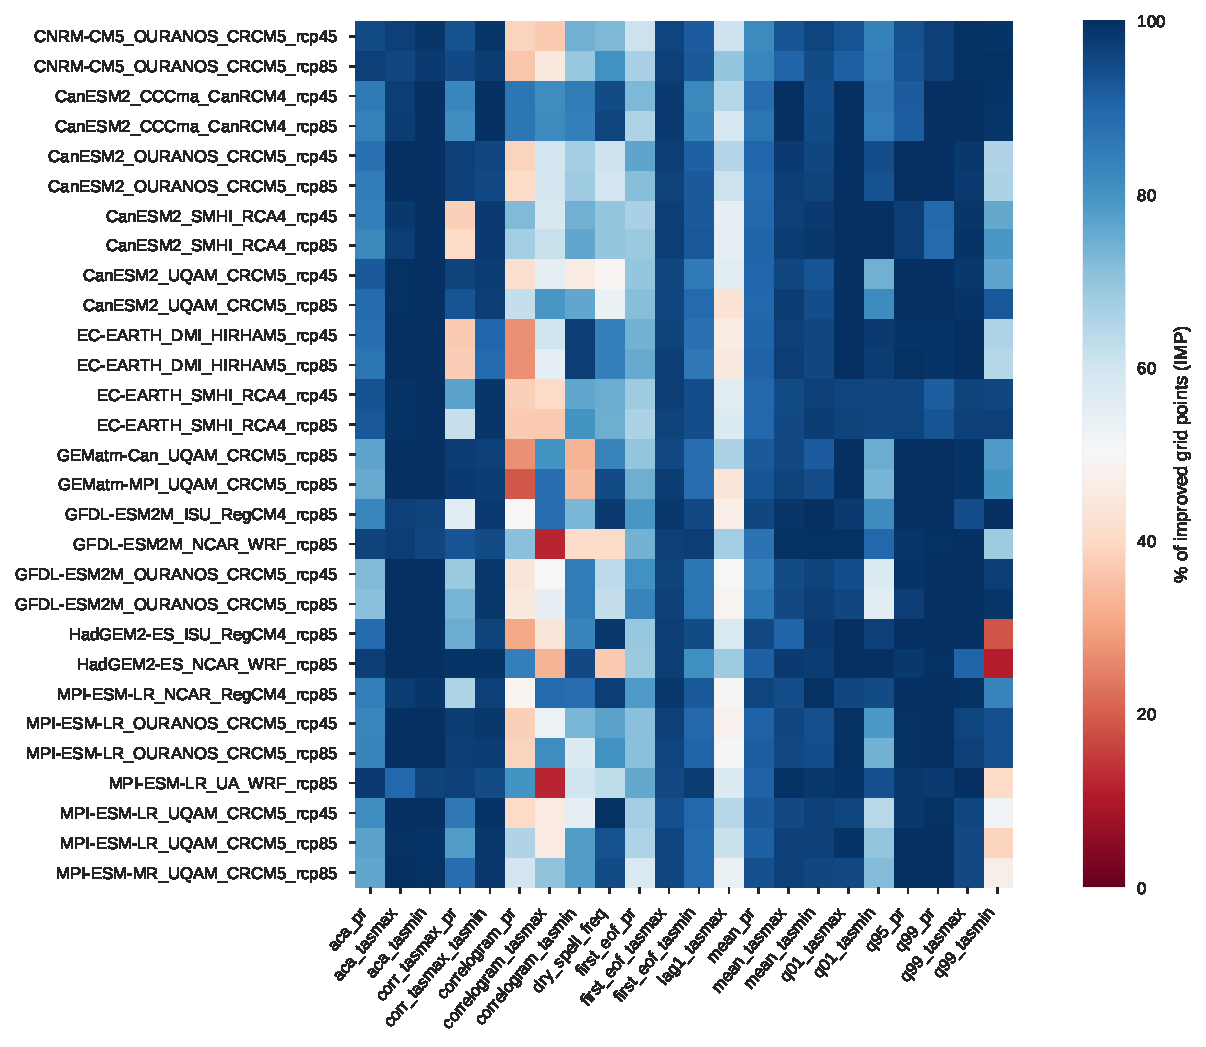
\includegraphics[width=\textwidth]{../images/overall_improvement.pdf}
    \caption{The proportion of improved gridpoints (IMP) for the Haudenausonee region.}\label{fig:imp}
\end{figure}

As always when asserting the quality of a bias-adjustment, one must not forget that terms like "improvement" and "performance" refer to the change in comparison with the reference which is taken as the "Truth" in this context.
Thus, the validity of bias-adjusted datasets are limited by the validity of the reference dataset.
A succinct analysis of ERA5-Land is detailed in the README at the root of this repository and provides the justification for using it as our reference.

This whole analysis not only serves as an assessment of the performance of ESPO-R5v1.0, but also as a benchmark for the next iterations of the ESPO datasets.
Here, we aim to test our performance evaluation tools and tune the list of properties for evaluation purposes.

The complete properties and measures dataset is too large to be delivered through a git repository, but we offer a sample here.
Values for most properties, and their measures, on the Haudenosaunee region are given in the \texttt{data/} folder.
Other regions and missing properties can be provided to interested parties on demand.

\section{Marginal aspects}\label{sec:marg}
Detrended Quantile Mapping will adjust most properties marked as "marginal" by construction.
Our algorithm divides the distribution of values for each day of the year into 50 bins and thus the percentile properties should look almost perfectly adjusted (see figure~\ref{fig:qq}).
Indeed, all members show over 90\% of improved grid points for the percentiles properties of pr and tasmax.
Oftentimes the non-improved grid points are those where the simulation was already comparing well with the reference.
This indicates that there is noise (variability) in the scenario and shows a limit in using this IMP metric.
This can also be seen when comparing results for members where the initial resolution was 0.44° with those for the 0.22° sources: the former systematically have stronger IMP scores than the latter;
However, we can't really conclude anything other than the observation that bilinear regridding is an inferior downscaling technique than a regional climate model.

\begin{figure}
\centering
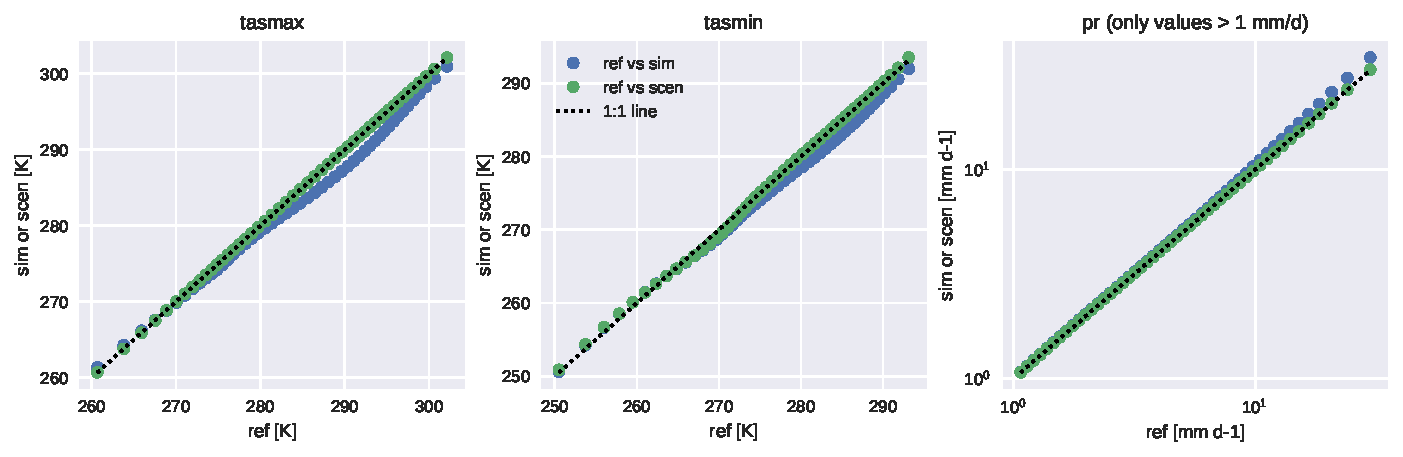
\includegraphics[width=\textwidth]{../images/QQplots.pdf}
\caption{Q-Q plots for member MPI-M-MPI-ESM UQAM-CRCM5 rcp45, including all points of the Haudenosaunee region. This member's source simulation was on the NAM-44 domain. Only wet days are included.}\label{fig:qq}
\end{figure}

Scores are lower for tasmin. Recall that here tasmin is not directly adjusted, but is rather computed from the adjusted tasmax and dtr, the daily temperature range.
This indirect adjustment seems to be visible when inspecting the properties and measures, as will be shown again further down.
Conclusions are very similar for the "mean" properties.

The dry spell frequency has a similar behaviour where only members with large initial biases show strong IMP.
This property is also somewhat adjusted by construction during the pre-processing of precipitation data, at least for members with too many dry days, when compared to the reference.
The process explained in the "Adjustment" document (section "Pre-processing of precipitation") is mostly meant to ensure valid quantile mappings, but it does have a small effect on the final scenarios.
There are still some members where the frequency of dry days is nearly 6\% higher in the scenarios then in the reference, especially over lakes.
The bias is also quite consistently positive for all members and regions.

\section{Temporal aspects}
As the bias adjustment acts separately on each day of the year and, as we've seen, the scenario distribution matches well with the reference, we expected that the annual cycle amplitude would be well adjusted.
And indeed, for both temperatures, the improvement is major for all members, most showing IMP values over 90 \%.
Scores are slightly weaker for precipitation, but it is important to note that in some regions precipitation doesn't have an annual cycle as strong nor as consistent as temperature.
Still, IMP values are over 75 \% for two-thirds of the members, and there is strong correlation between the improvement amount and the initial bias.
Some members showed severely inadequate annual cycle amplitude patterns before the adjustment, which makes their high IMP scores almost trivial;
So much so that it becomes less a measure of the performance of the bias adjustment than a measure of the bias between the simulation and the reference, see figure~\ref{fig:acapr} for example.

\begin{figure}
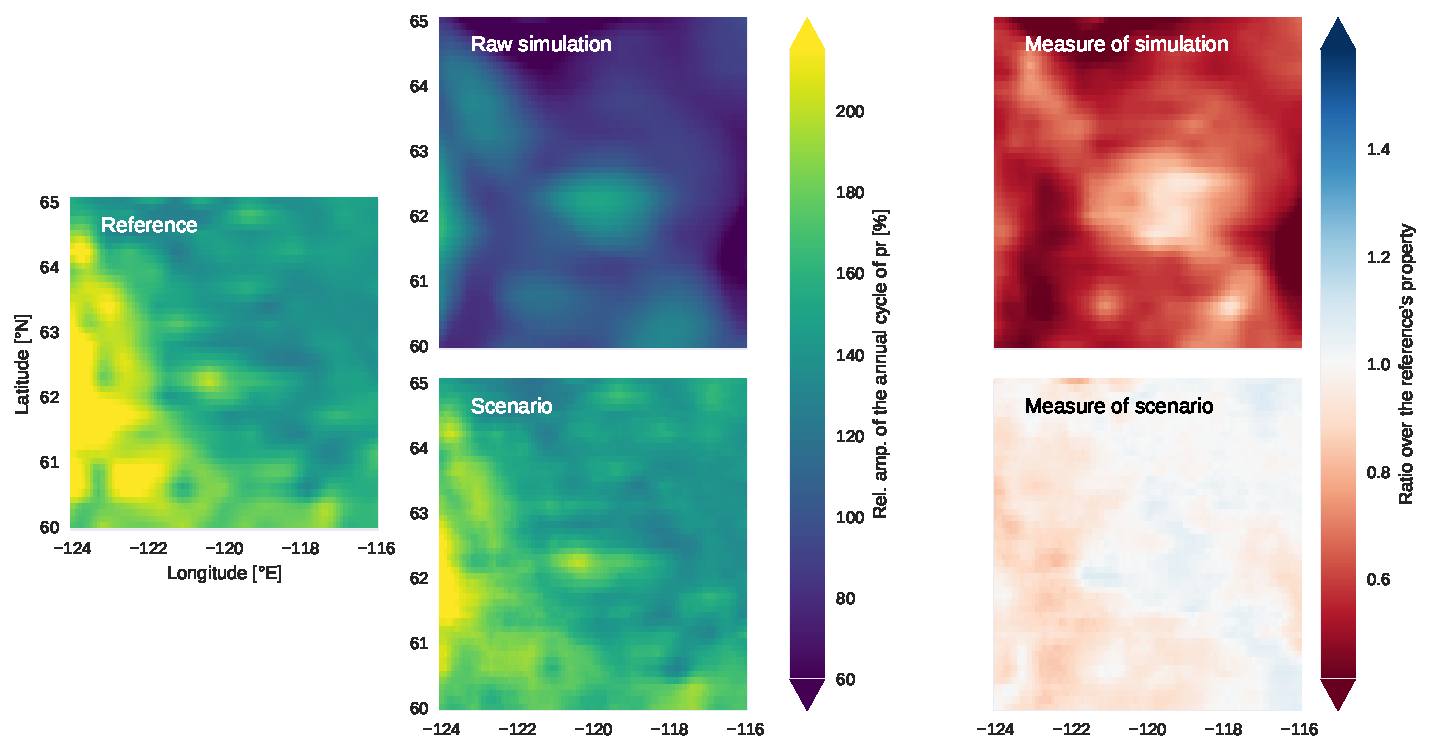
\includegraphics[width=\textwidth]{../images/aca_pr_diags.pdf}
\caption{Relative amplitude of the annual cycle of precipitation ICHEC-EC-EARTH DMI-HIRHAM5 rcp45, 1981-2010, Dene region. This example of diagnostic maps showing a large bias between the simulation and the reference as well as a large improvements in the scenario. This case has a IMP value of 88\%.}\label{fig:acapr}
\end{figure}

Unsurprisingly, the lag-1 autocorrelation property doesn't seem to be significantly improved by the bias-adjustment.
Generally, the lag-1 autocorrelation structure from the simulations is almost identical in the scenarios.
Indeed, the algorithm does not adjust this aspect explicitly, but it may be interesting for future versions of the ESPO datasets to address this issue.

\section{Multivariate aspects}
Our algorithm is inherently univariate, but the special treatment of tasmin does seem to have a strong effect on the correlation between tasmax and this variable.
Most simulations of the ESPO-R5 ensemble tend to underestimate the correlation between the two variables and this bias is drastically reduced in the scenarios.
If our analysis is correct, the reconstruction of tasmin from dtr and tasmax does improve that aspect of the data, while reducing the improvement of other properties, as discussed above (section \ref{sec:marg}).

When looking at the biases in the tasmax-pr correlation, we do see large IMP values in some regions and members.
In most of these cases, the initial bias between the simulations and the reference was quite large (much larger than in the tasmax-tasmin case), which leaves much room for improvement.
This is visible as a strong correlation between the improvement of the measure in the scenario and its value in the simulation.
In other cases, the improvement is less clear with IMP values around 50\%.
Figure~\ref{fig:icorr} shows such a case, but it reveals a pattern created by the bilinear interpolation used when regridding the simulations to the reference grid.
The pattern gets smoothed out by the bias adjustment, but it is replaced by another one inherited from the reference itself, at least in the case of this particular property.

\begin{figure}
    \centering
    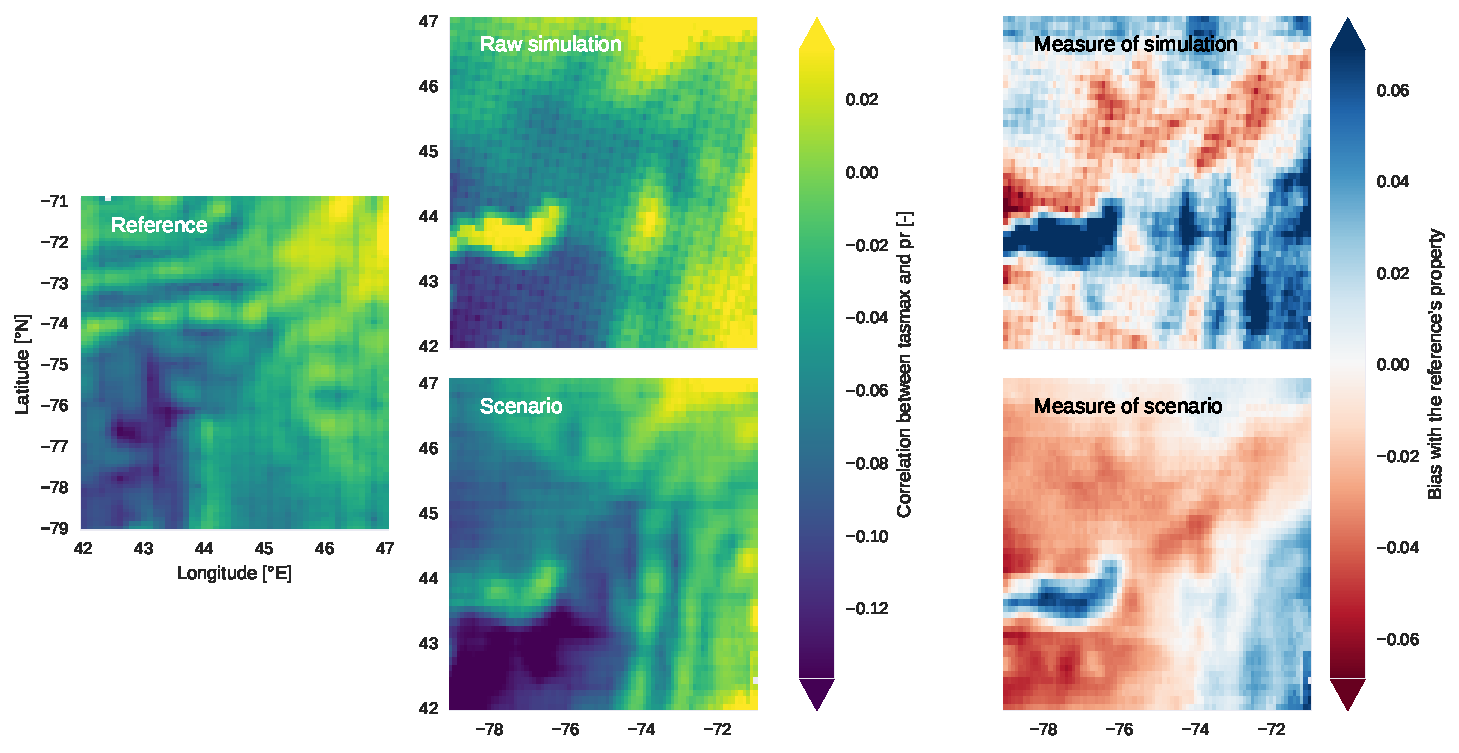
\includegraphics[width=\textwidth]{../images/corr_tasmax_pr_diags.pdf}
    \caption{Intervariable correlation (Spearman rank-order) between tasmax and pr for GFDL-ESM2M ISU-RegCM4 rcp85, 1981-2010 period, Haudenosaunee region. This case has a IMP value of 55\%}\label{fig:icorr}
\end{figure}

\section{Spatial aspects}
Despite the lack of real benchmark values, the spatial correlograms seem to visually show an already good fit between the simulations and the reference, though we see no improvement in the scenarios.
In general, the correlogram are very similar between the simulations and the scenarios and we see no significant change in the spatial correlation length (distance where the correlation drops below a certain threshold, taken here as 0.35 for all variables).
Figure~\ref{fig:scorr} shows an example where the bias is quite large (compared to those of other members of the ensemble).
Although we explicitly take care of adjusting the dry days frequency, we do not see the spatial correlation improvement described by \cite{Francois2020}.

\begin{figure}
\centering
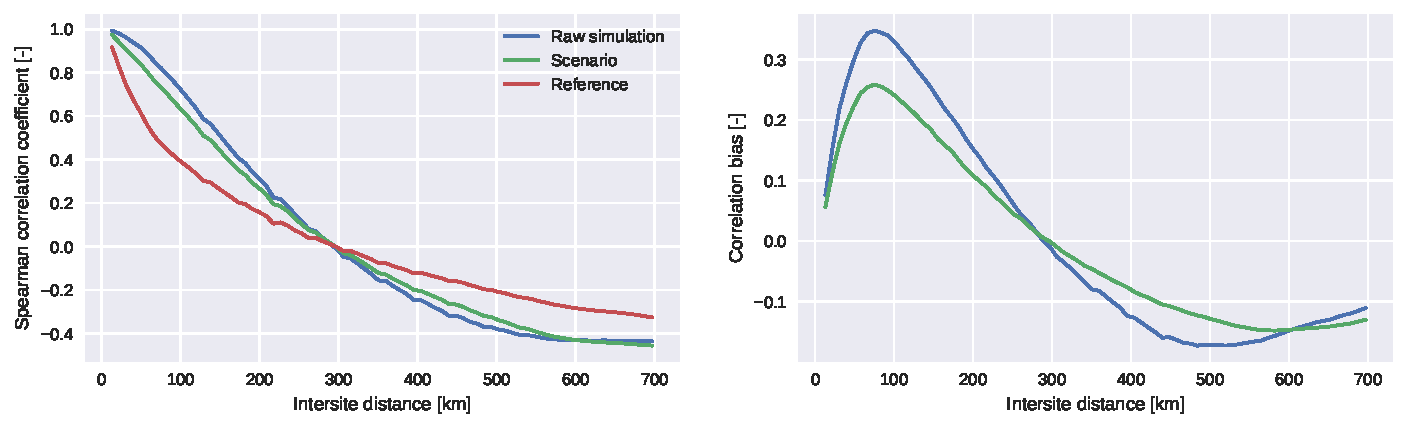
\includegraphics[width=\textwidth]{../images/correlogram_tasmin_diags.pdf}
\caption{Correlogram for tasmin, member ICHEC-EC-EARTH DMI-HIRHAM5 rcp 4.5, Ute region, 1981-2010.}\label{fig:scorr}
\end{figure}

\section{Climate change signal}
Nothing much is to be said about the effect of the bias adjustment on the climate change signal since it is preserved by construction.
The use of a LOESS detrending with a 30-year window on each day of year preserves the mean change in the variables as simulated by the regional models.
If we look at 30-year means of the variable, as is often done in climate change studies, there is no difference between the raw simulations and their adjusted scenarios (not shown).

\section{Ensemble variability}
Figure~\ref{fig:ensvar} shows the annual timeseries of two indices, the average daily maximal temperature and the total precipitation.
The indices are given as change from the 1981-2010 period mean, which allows us to see that the bias-adjustment did not change the ensemble spread in a significant way.
We infer this to signify that the inter-annual variability of each member was preserved.

\begin{figure}
\centering
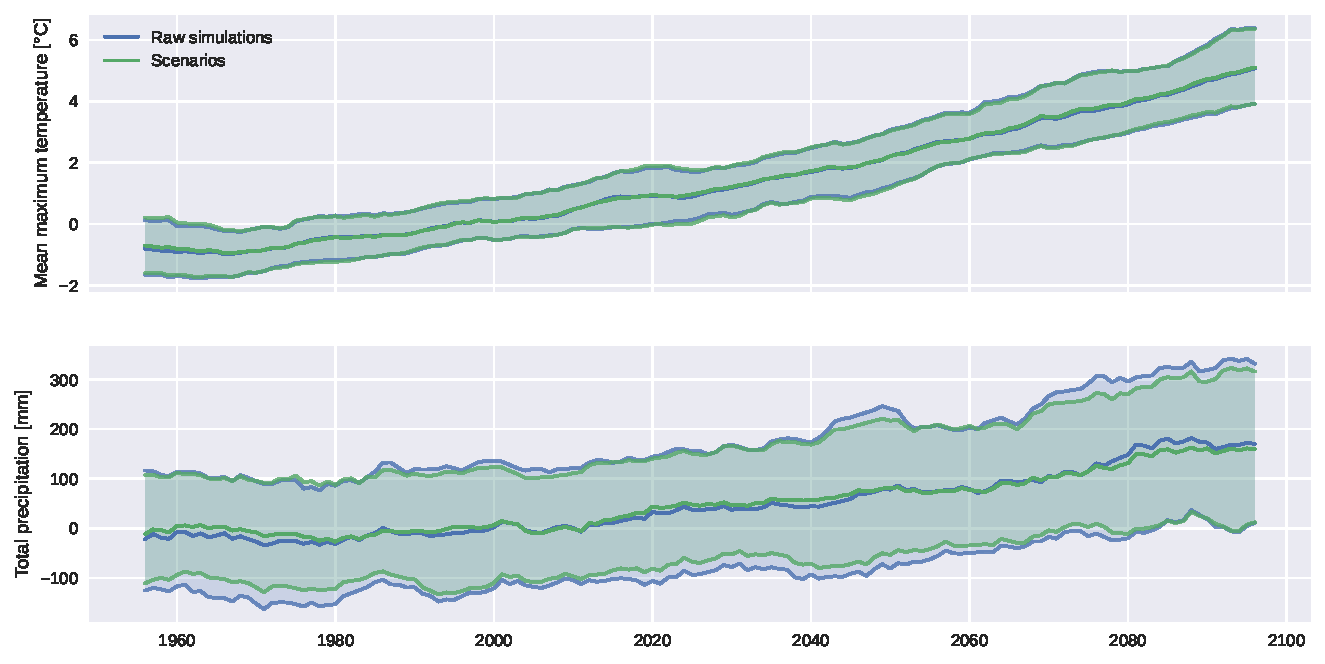
\includegraphics[width=\textwidth]{../images/ensemble_variability.pdf}
\caption{Ensemble spread of the change in two annual indices. Change computed with reference to the 1981-2010 period mean. The lines are smoothed with a 10-year moving window.}\label{fig:ensvar}
\end{figure}

\begin{thebibliography}{6}
\bibitem[FV20]{Francois2020} François, B., Vrac, M., Cannon, A. J., Robin, Y., \& Allard, D. (2020). Multivariate bias corrections of climate simulations: Which benefits for which losses? Earth System Dynamics, 11(2), 537–562. https://doi.org/10.5194/esd-11-537-2020

\bibitem[MW15]{Maraun2015} Maraun, D., Widmann, M., Gutiérrez, J. M., Kotlarski, S., Chandler, R. E., Hertig, E., Wibig, J., Huth, R., \& Wilcke, R. A. I. (2015). VALUE: A framework to validate downscaling approaches for climate change studies. Earth’s Future, 3(1), 1–14. https://doi.org/10.1002/2014EF000259

\bibitem[V18]{Vrac2018} Vrac, M. (2018). Multivariate bias adjustment of high-dimensional climate simulations: The Rank Resampling for Distributions and Dependences (R2D2) bias correction. Hydrology and Earth System Sciences. https://doi.org/10.5194/HESS-22-3175-2018
\end{thebibliography}
\end{document}